\section{Our method} 
	In this section, we present our Sampling-based AMST(Approximate Minimum Spanning Tree) approach. To improve the efficiency, we employ cover tree data structure to compute the nearest neighbors.
	\subsection{Our New Sampling method}
		\begin{algorithm}
		  \caption{our first Sampling-based MST algorithm}  
			\KwIn{a set of N data points}
			\KwOut{an MST}
			 compute all nearest neighbors of data sets\;
			 sampling from the data sets by using the nearest neighbor\;
			 construct an MST of sampler points\;
			 insert the remained point to MST\;
		\end{algorithm}

		\begin{figure}[!t]
	        \centering
	        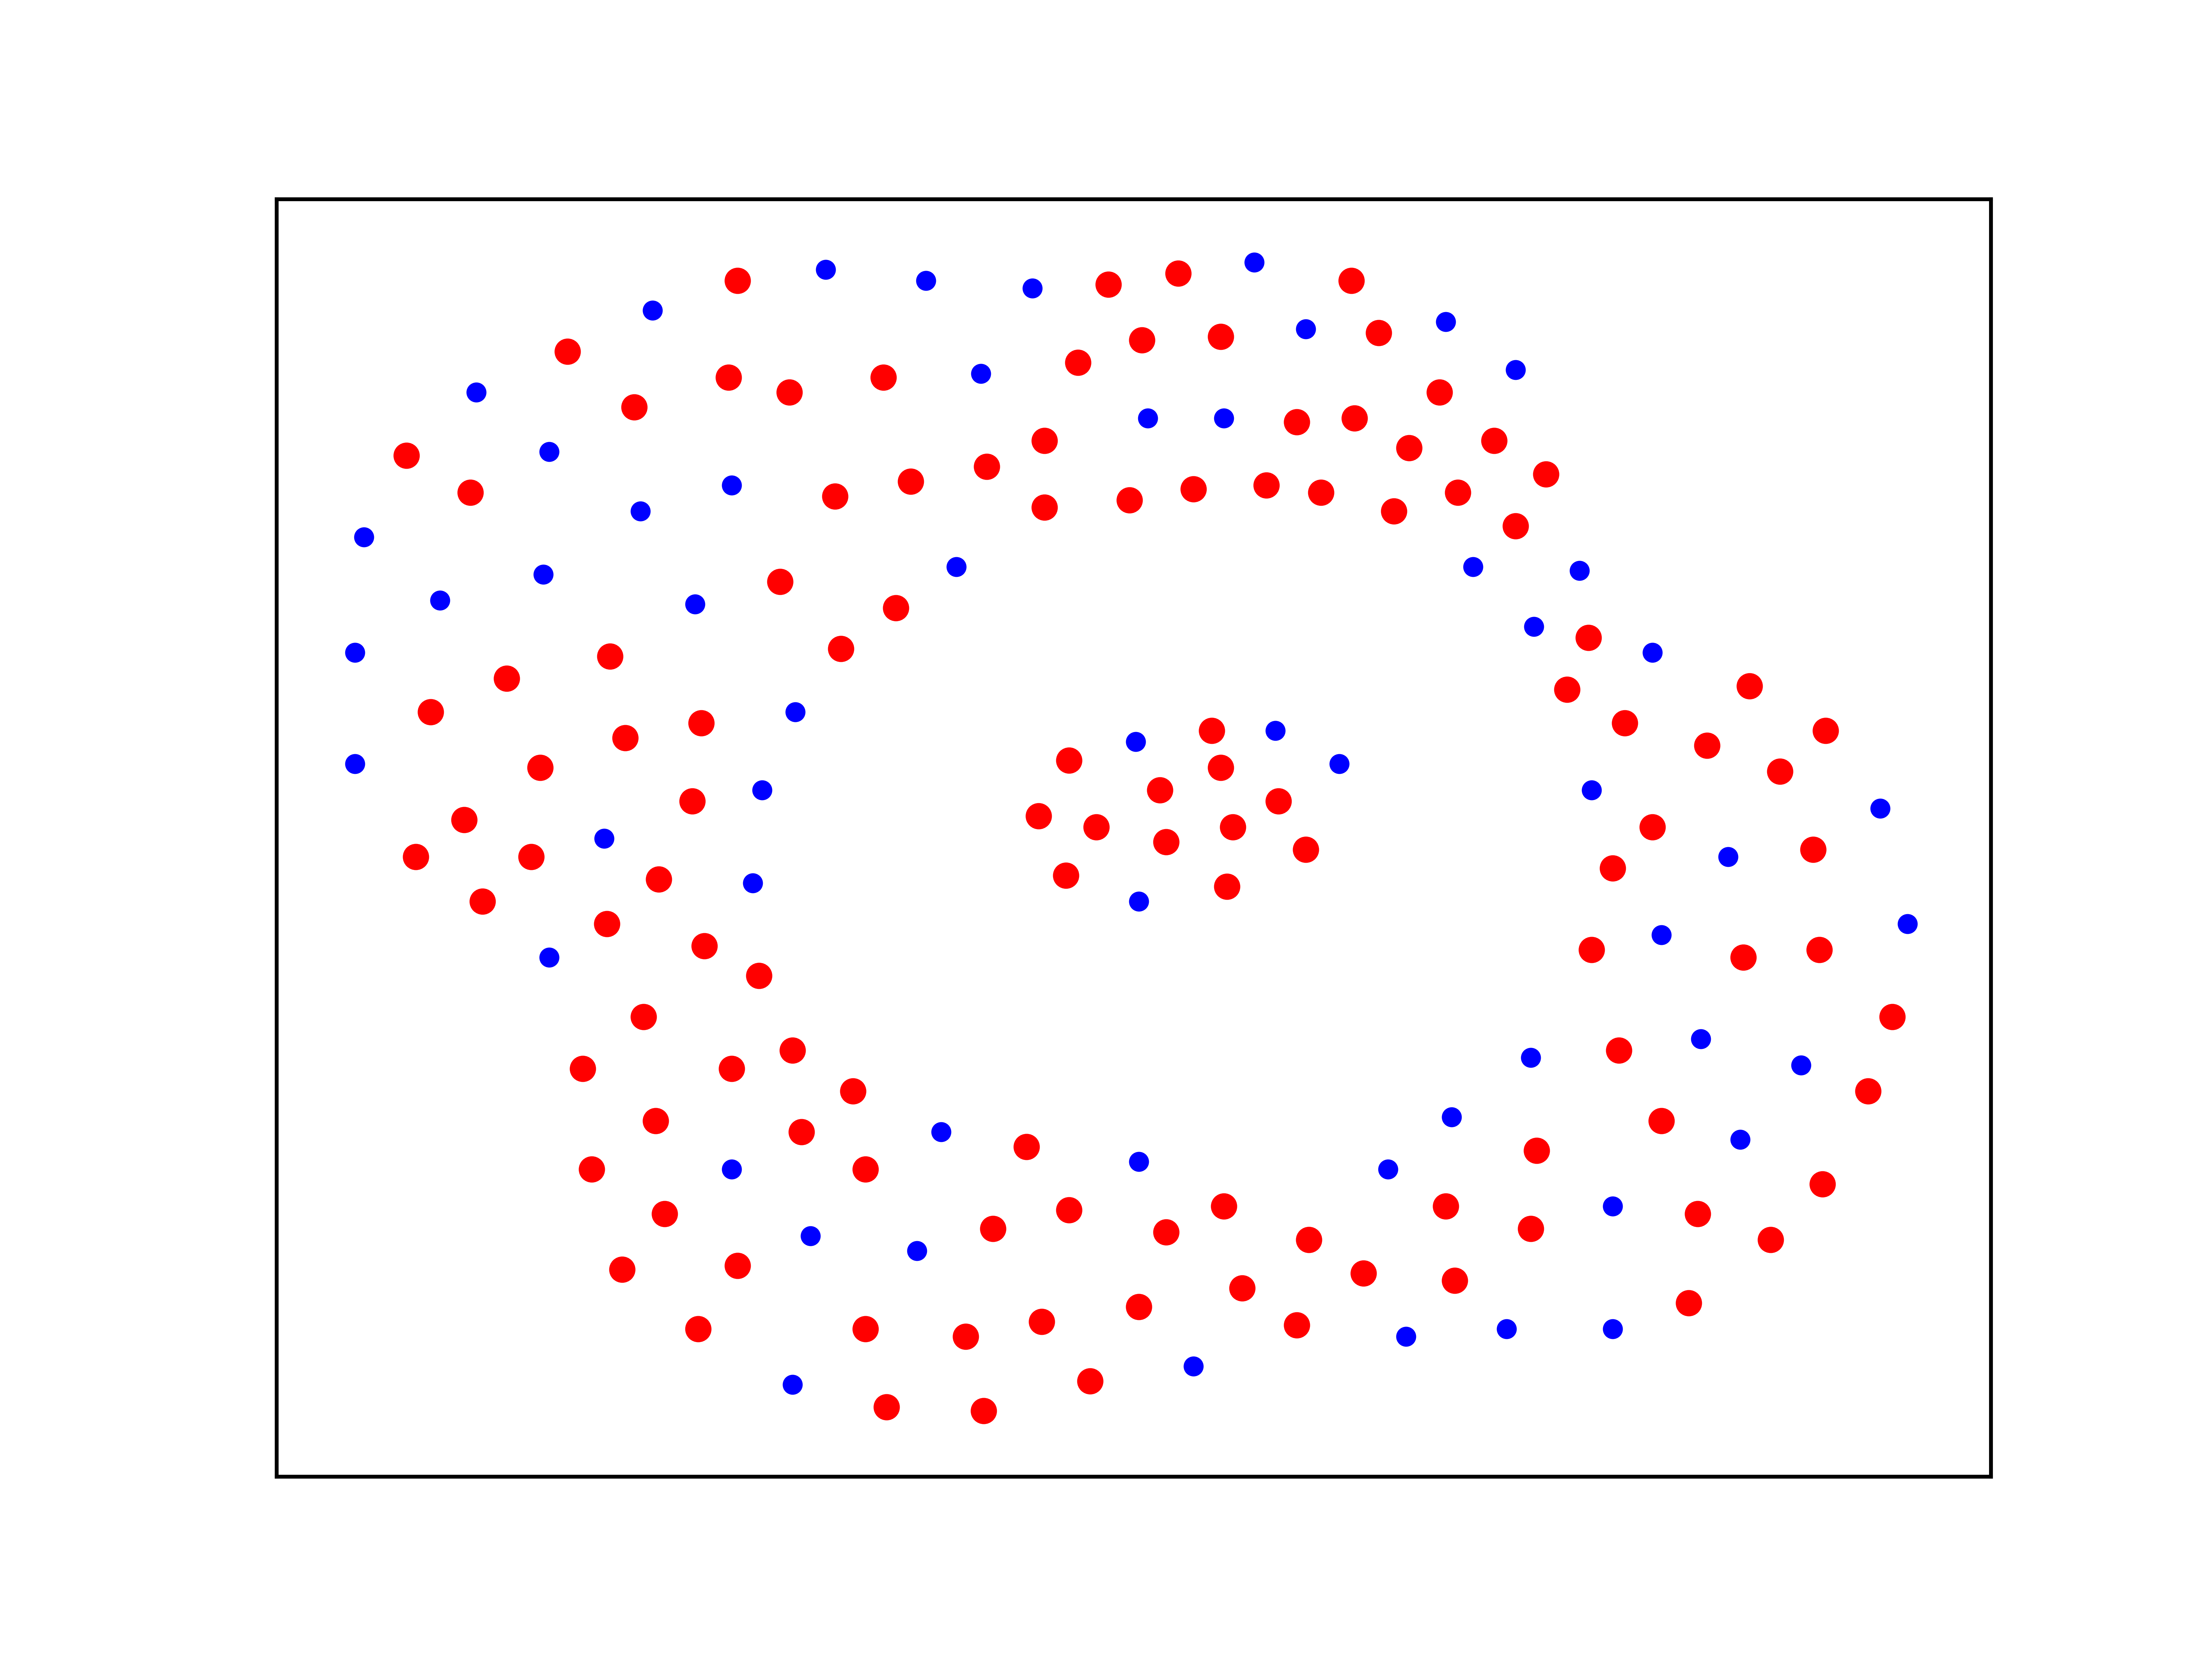
\includegraphics[width=0.43\linewidth]{1_step1.png}
	        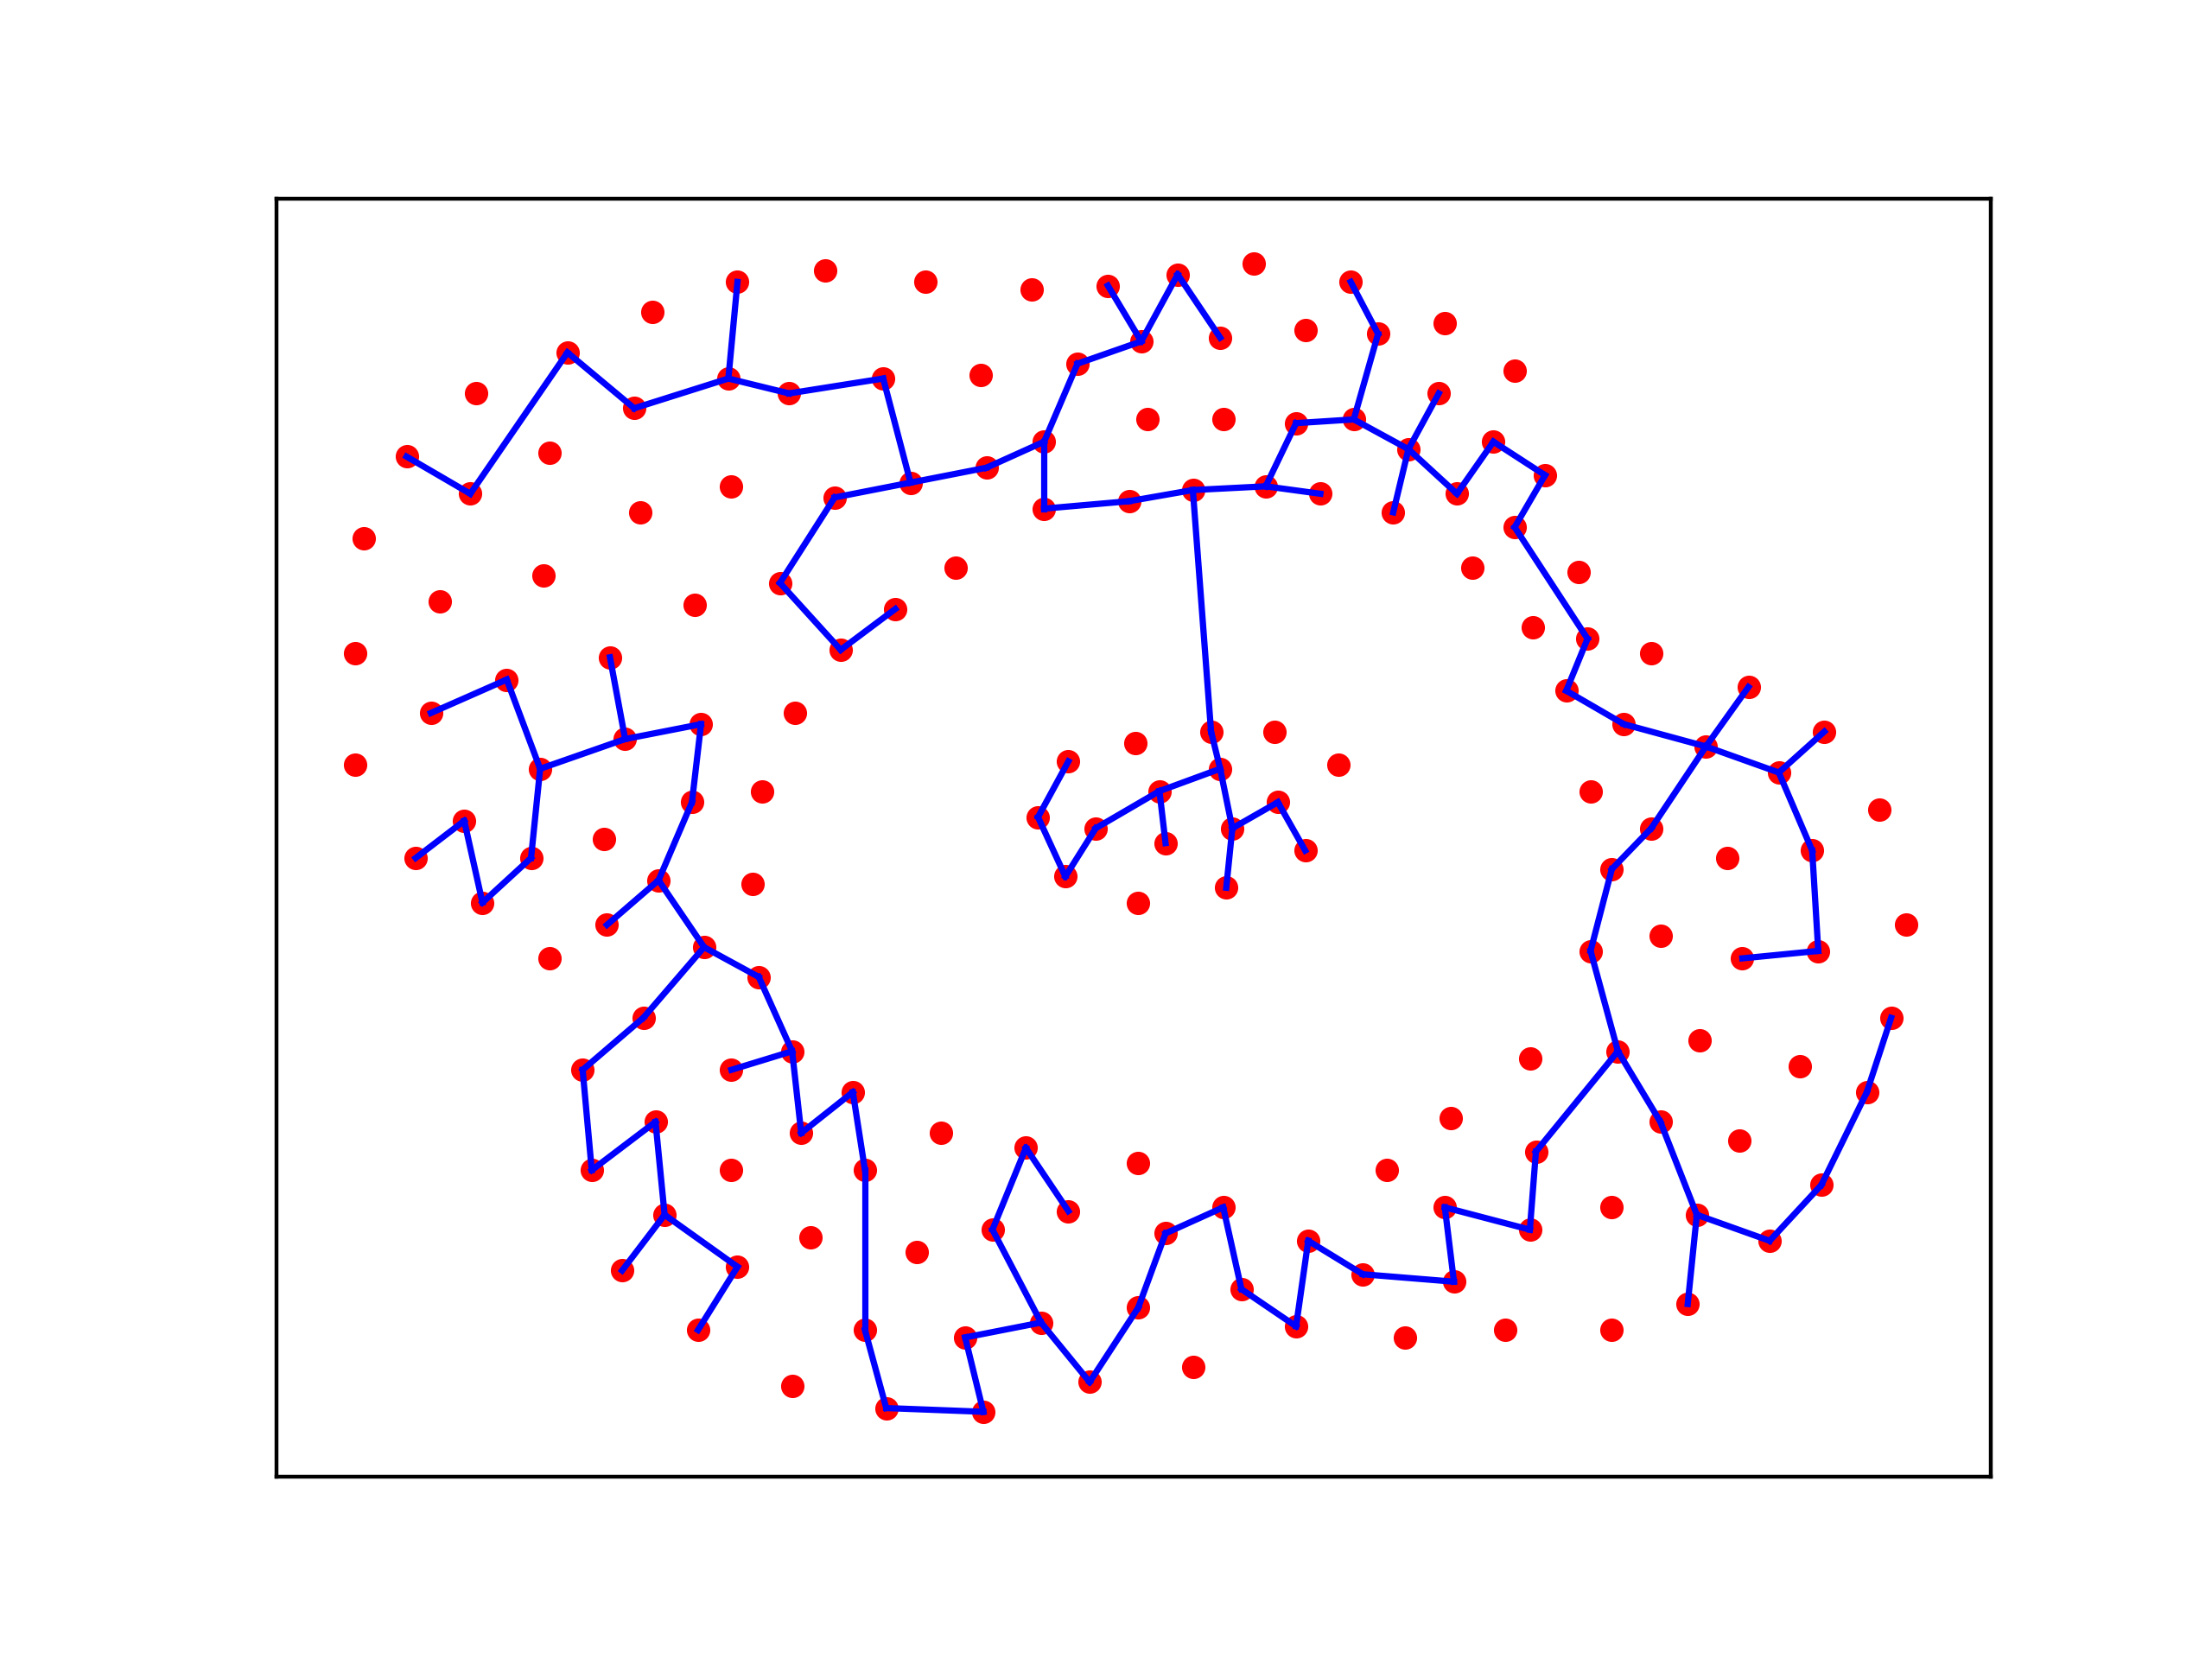
\includegraphics[width=0.43\linewidth]{1_step2.png}
	        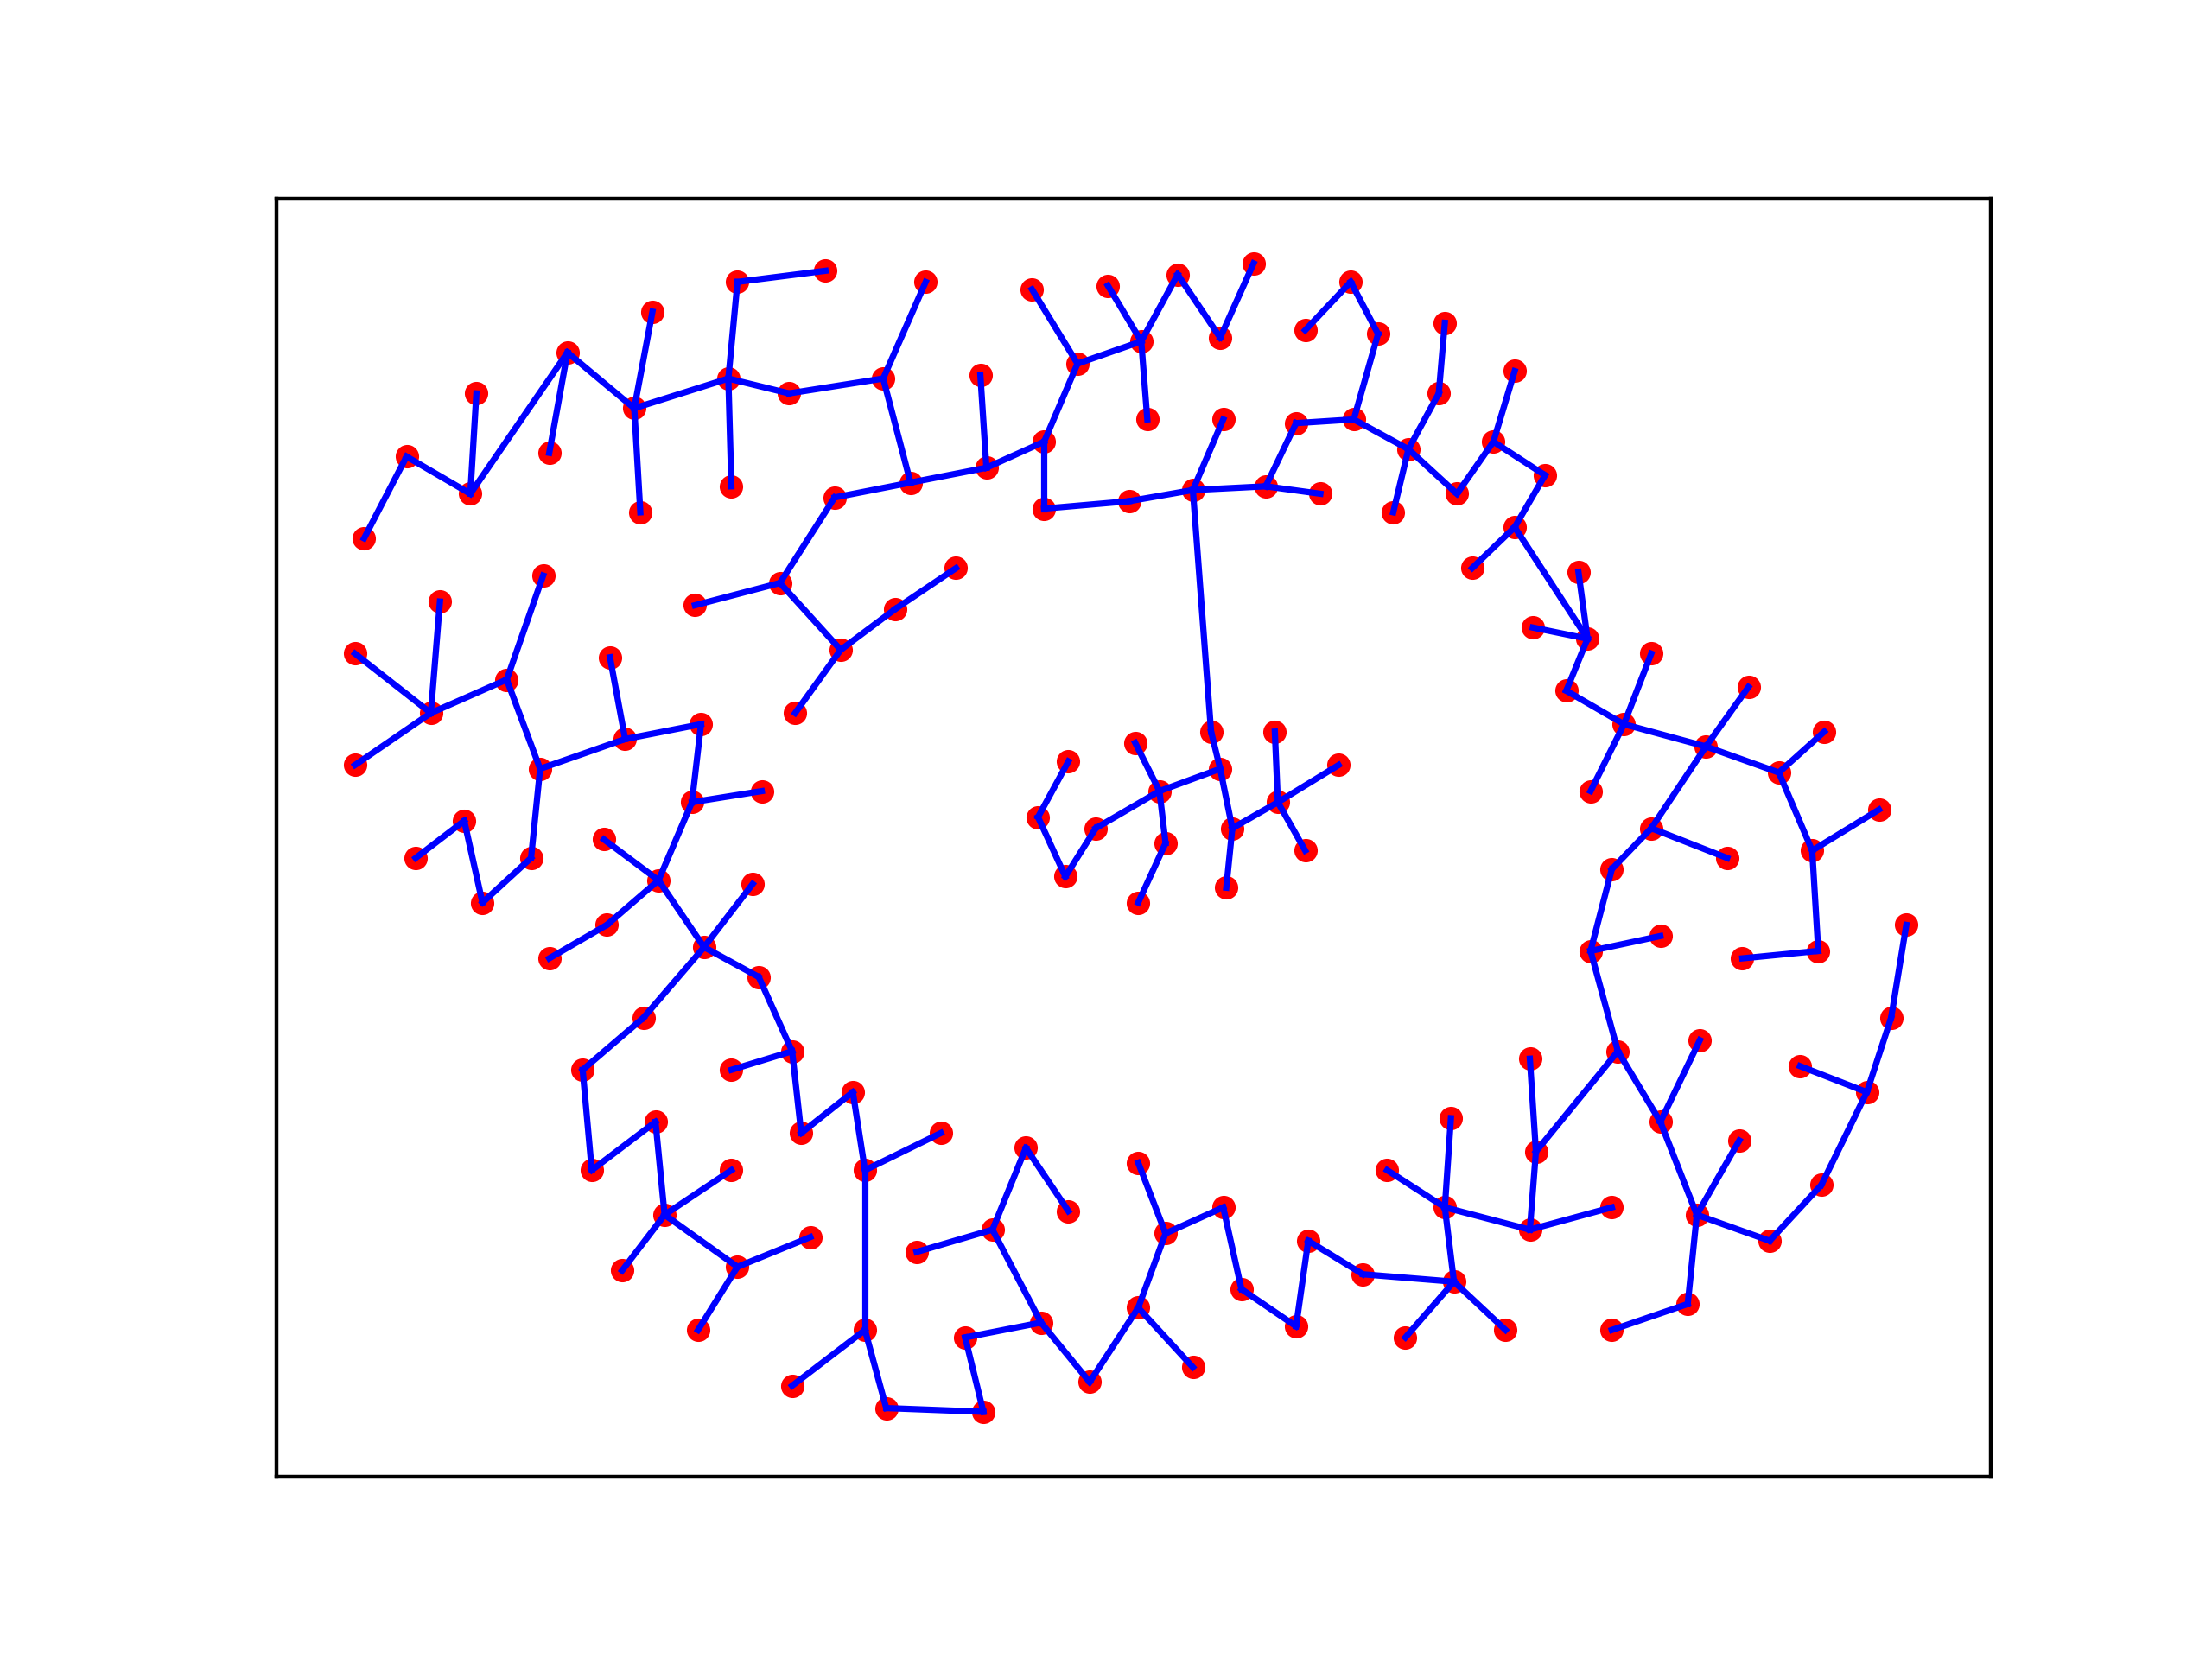
\includegraphics[width=0.43\linewidth]{1_step3.png}
	        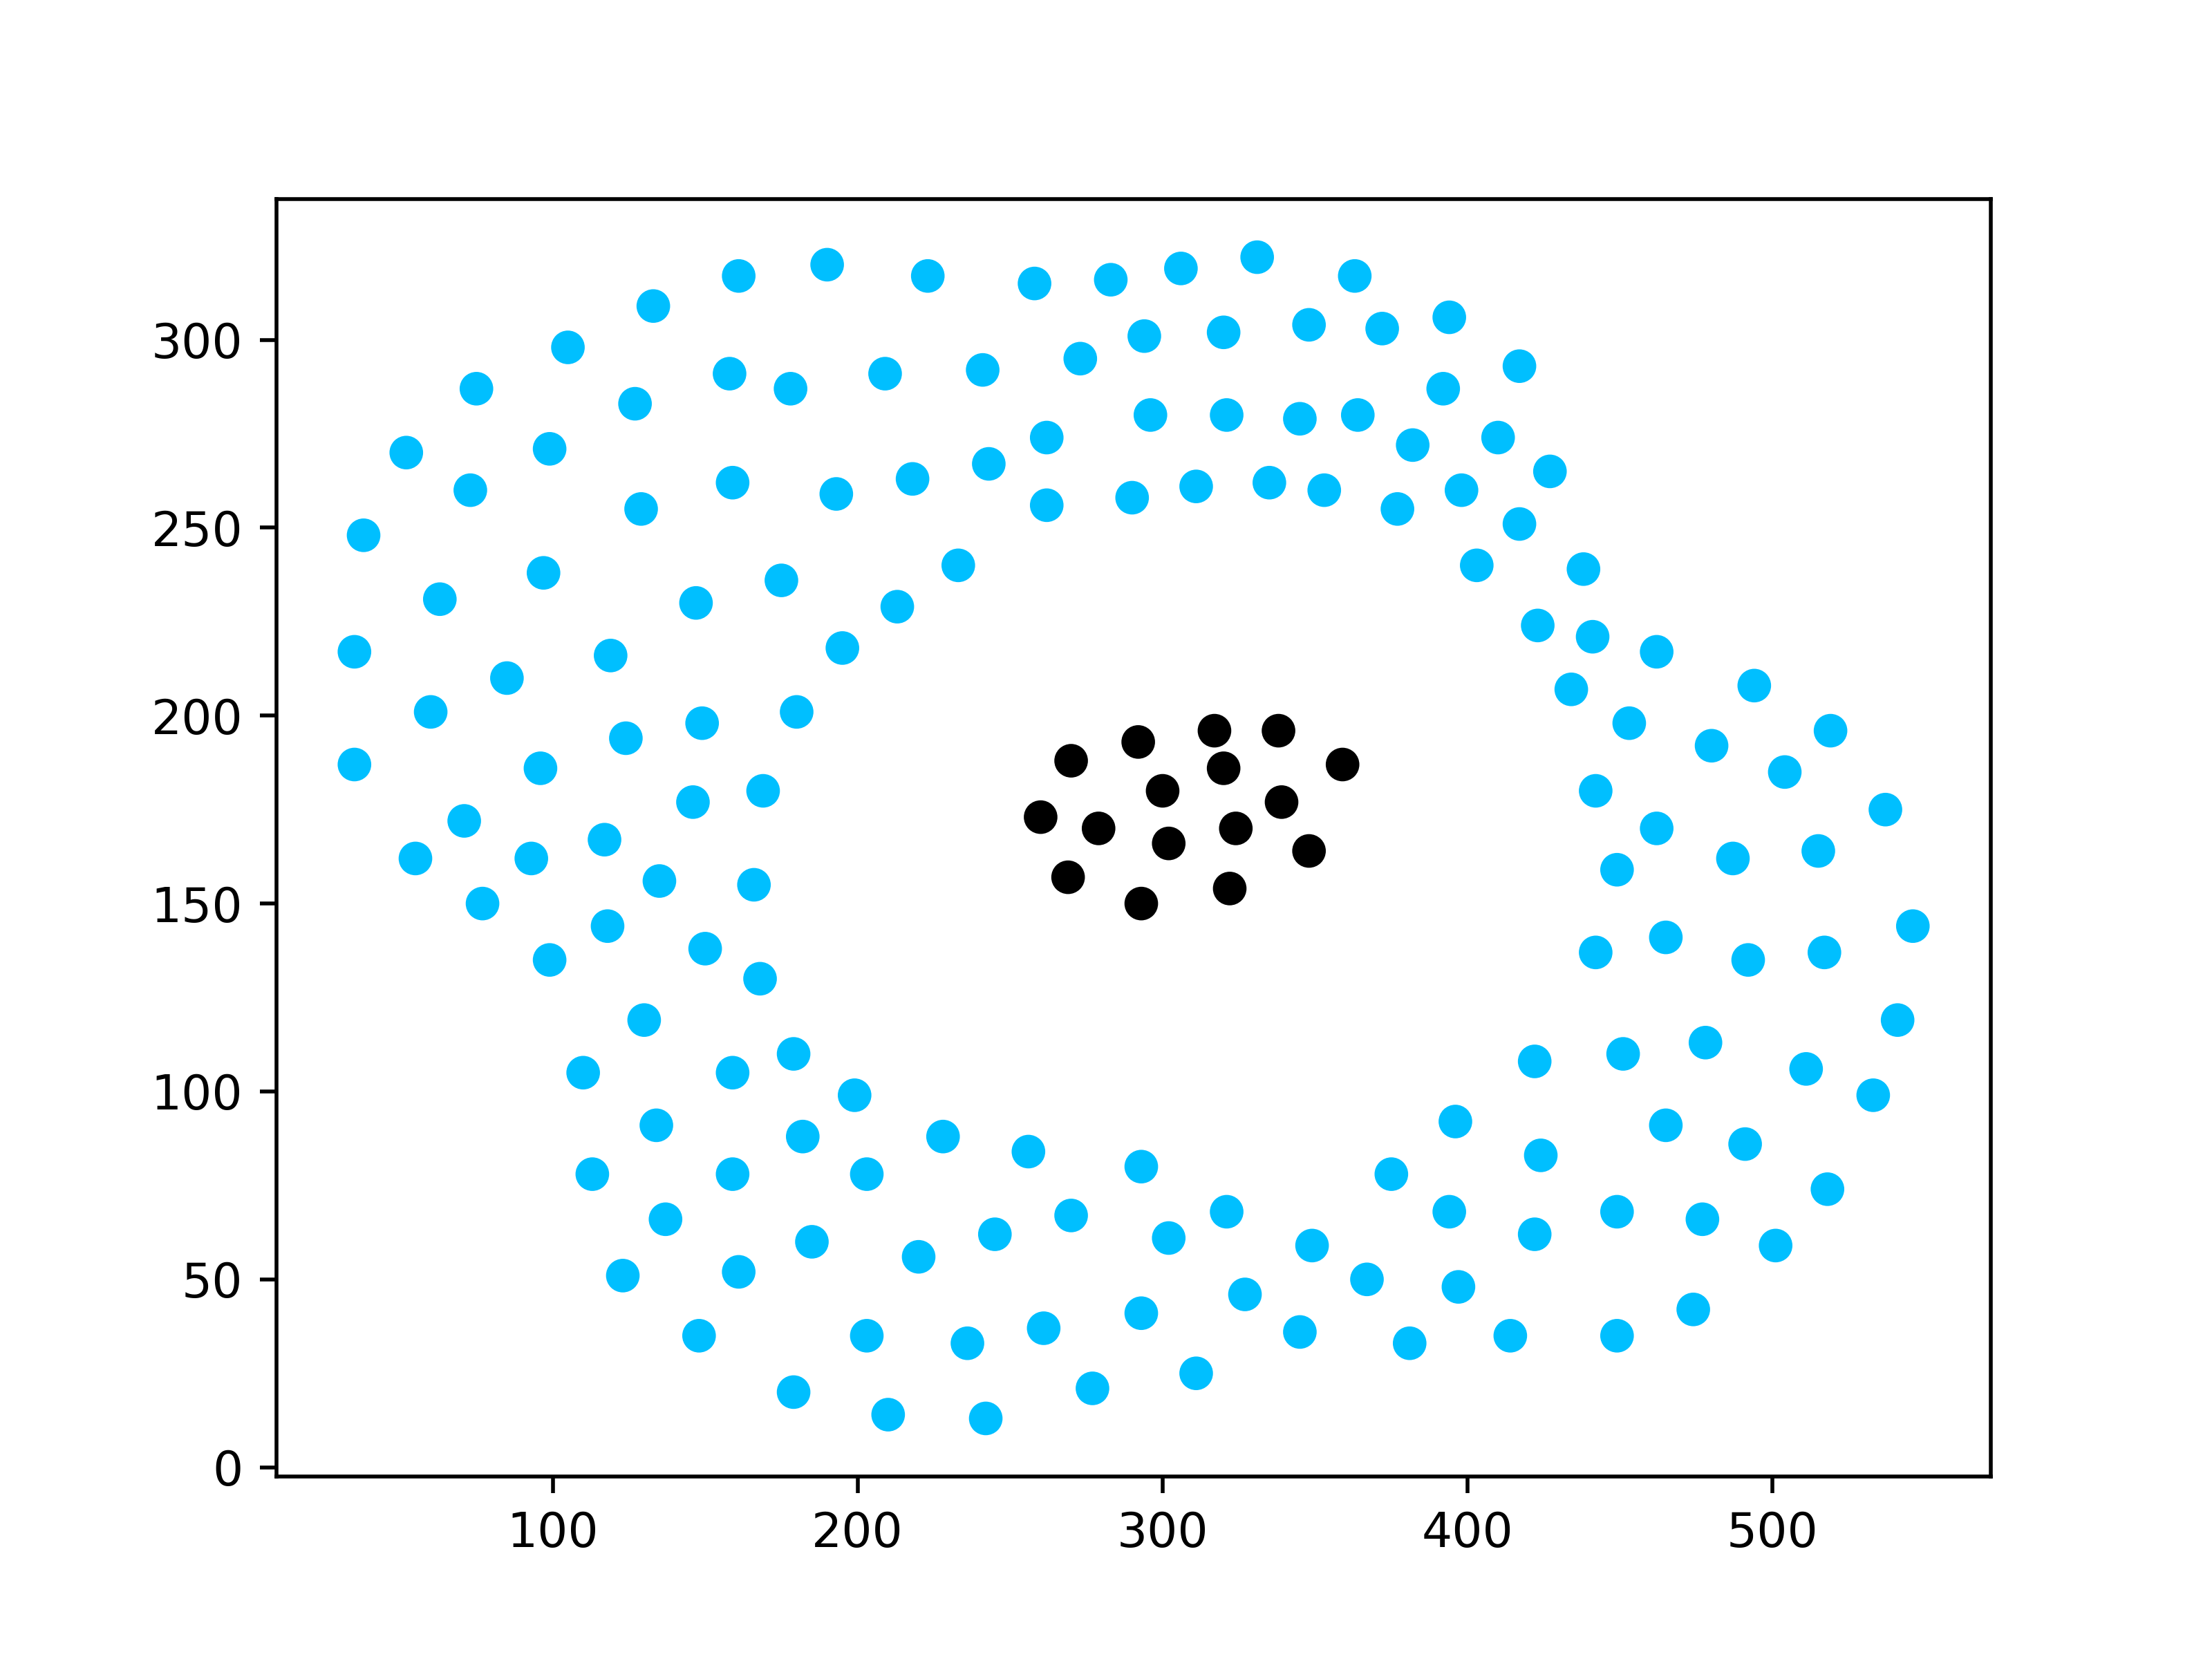
\includegraphics[width=0.43\linewidth]{1_step4.png}
	        \caption{steps of our second Sampling-based MST algorithm}
	    \end{figure}

		\begin{algorithm}
		  \caption{our second Sampling-based MST algorithm}  
			\KwIn{a set of N data points}
			\KwOut{an MST}
			 compute k nearest neighbors of data sets, where k=5\;
			 initialize the sampler points by the whole data sets\;
			 select one point as the start point, retain the nearest neighbor in the samplers and detele the other four neighbors\;
			 traverse the data sets until all neighbors are processed\;
			 construct graph with remained point by connecting them with their nearest neighbors\;
			 refine MST by connecting the single component and delete the longest edges by using Union Find sets\;
		\end{algorithm}
	
		\begin{figure}[!t]
	        \centering
	        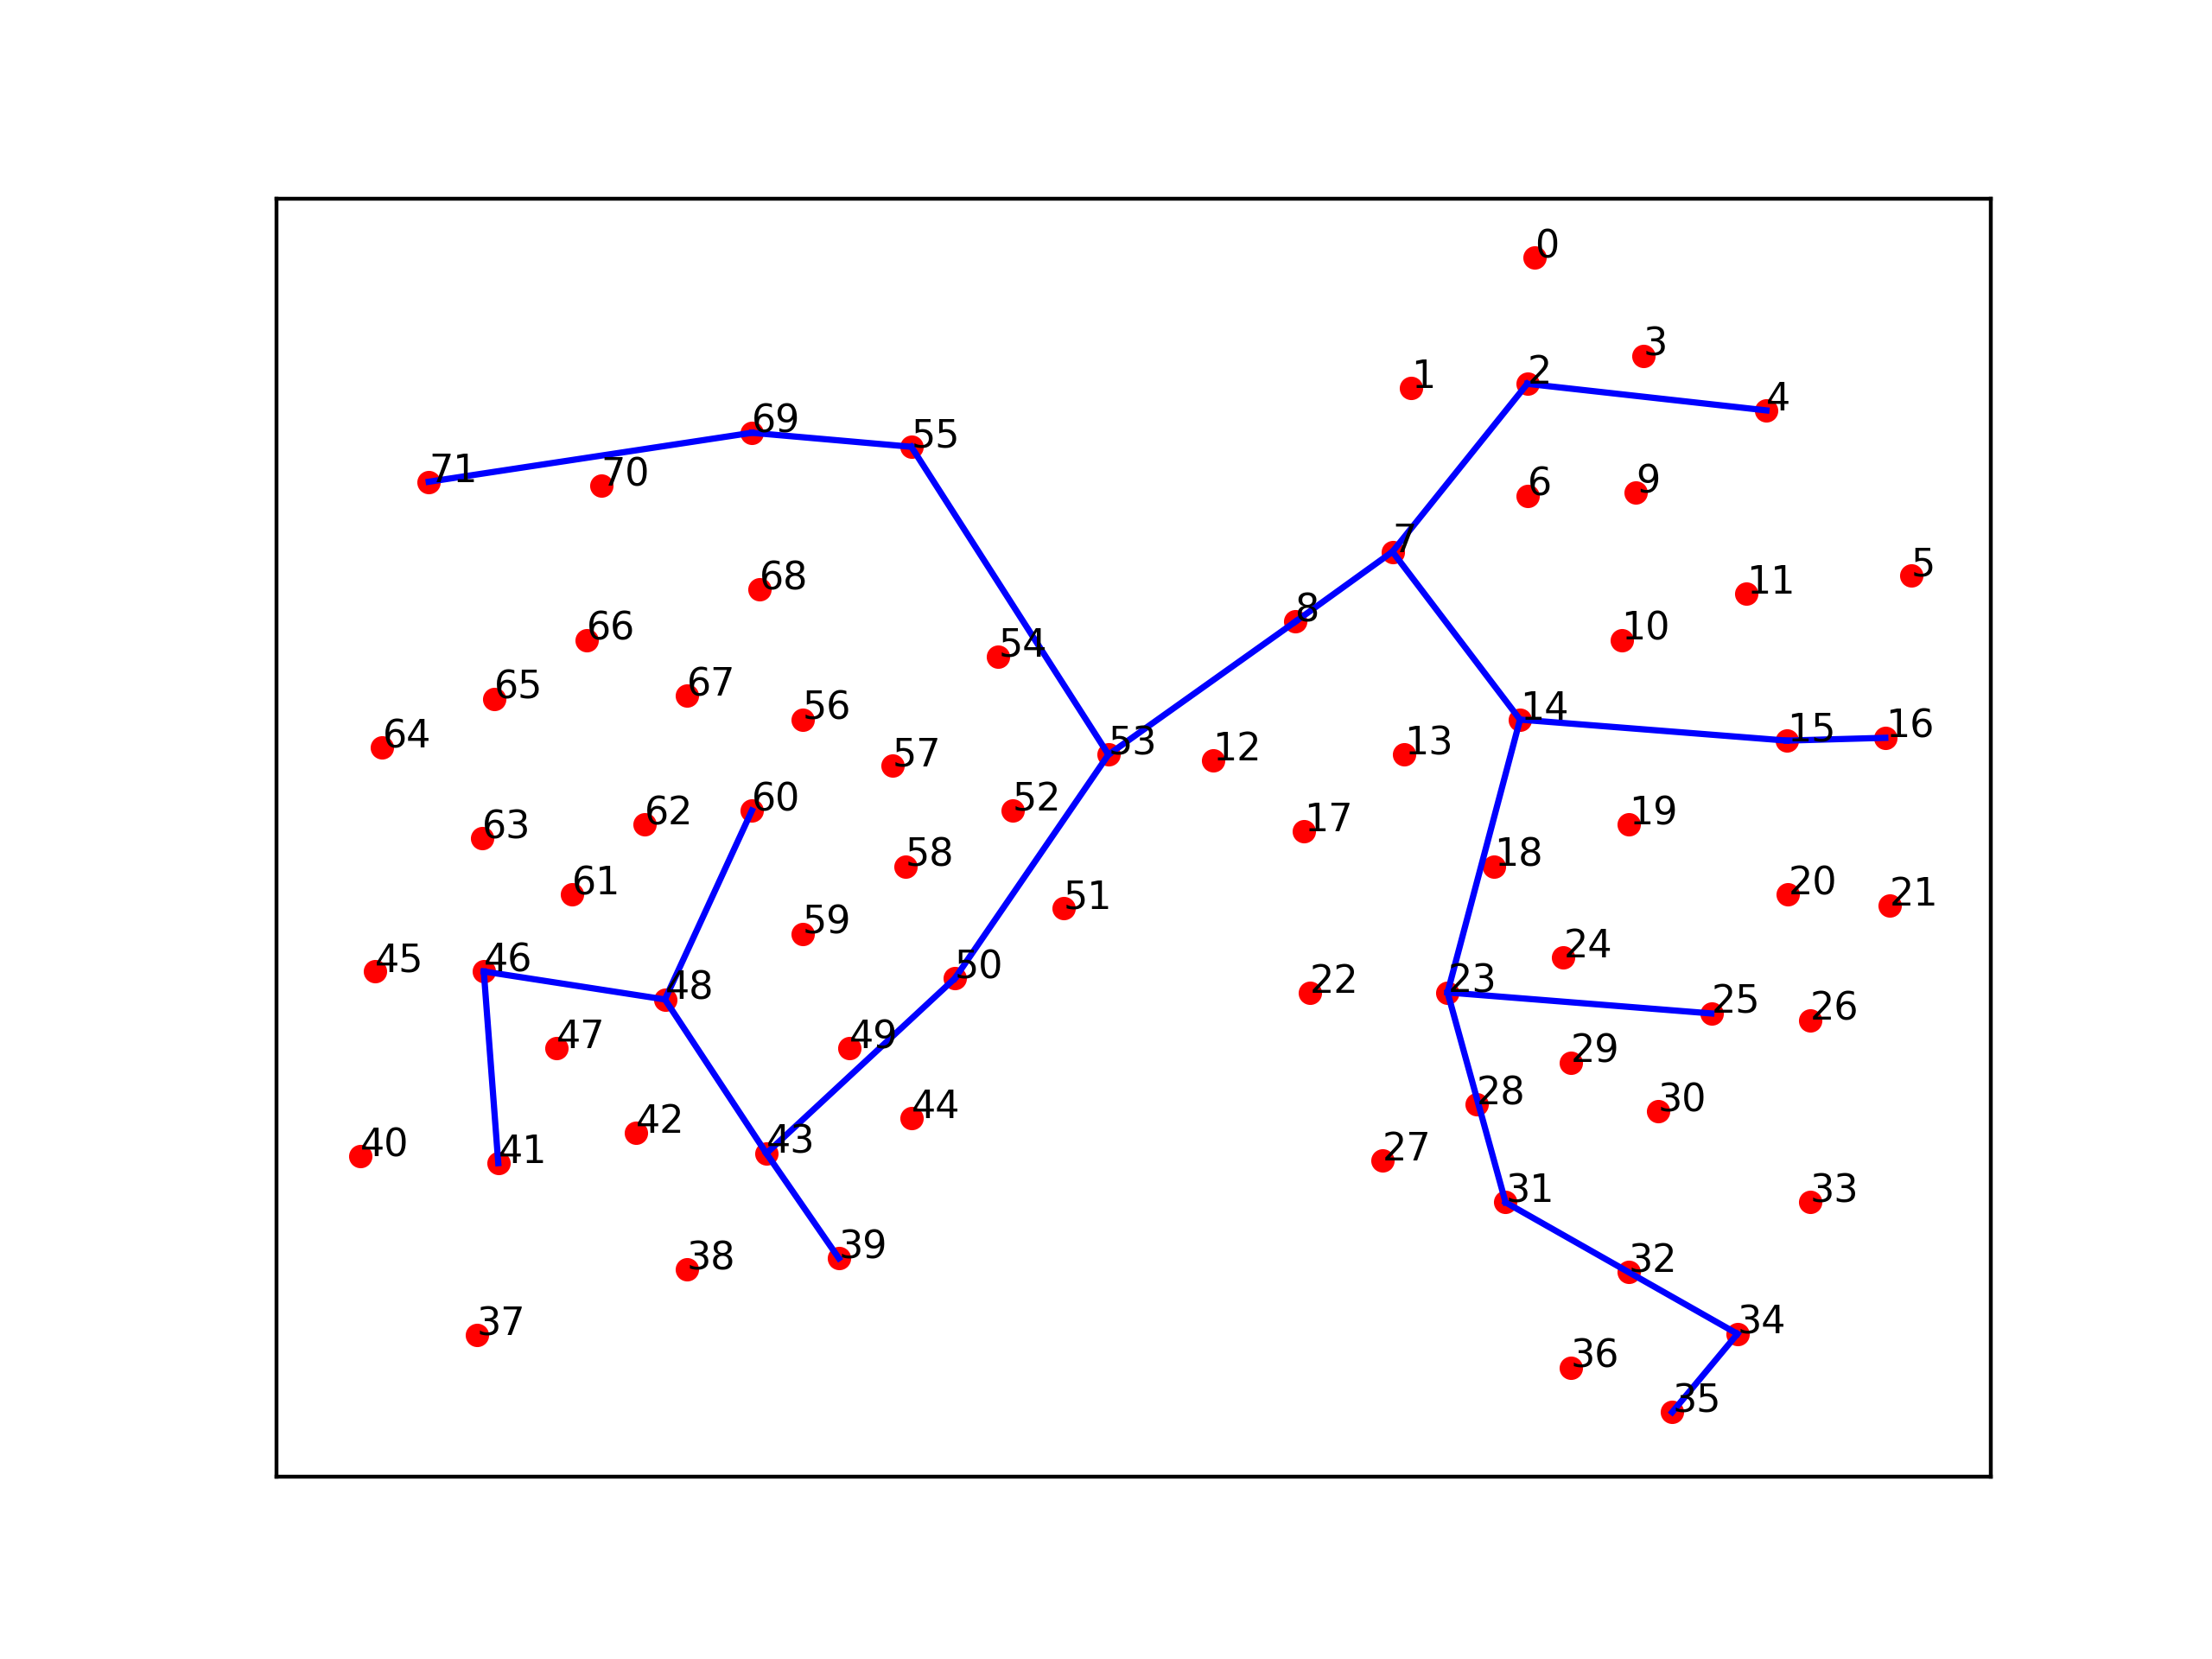
\includegraphics[scale=.5]{2_step1.png}\vspace{4pt}
	        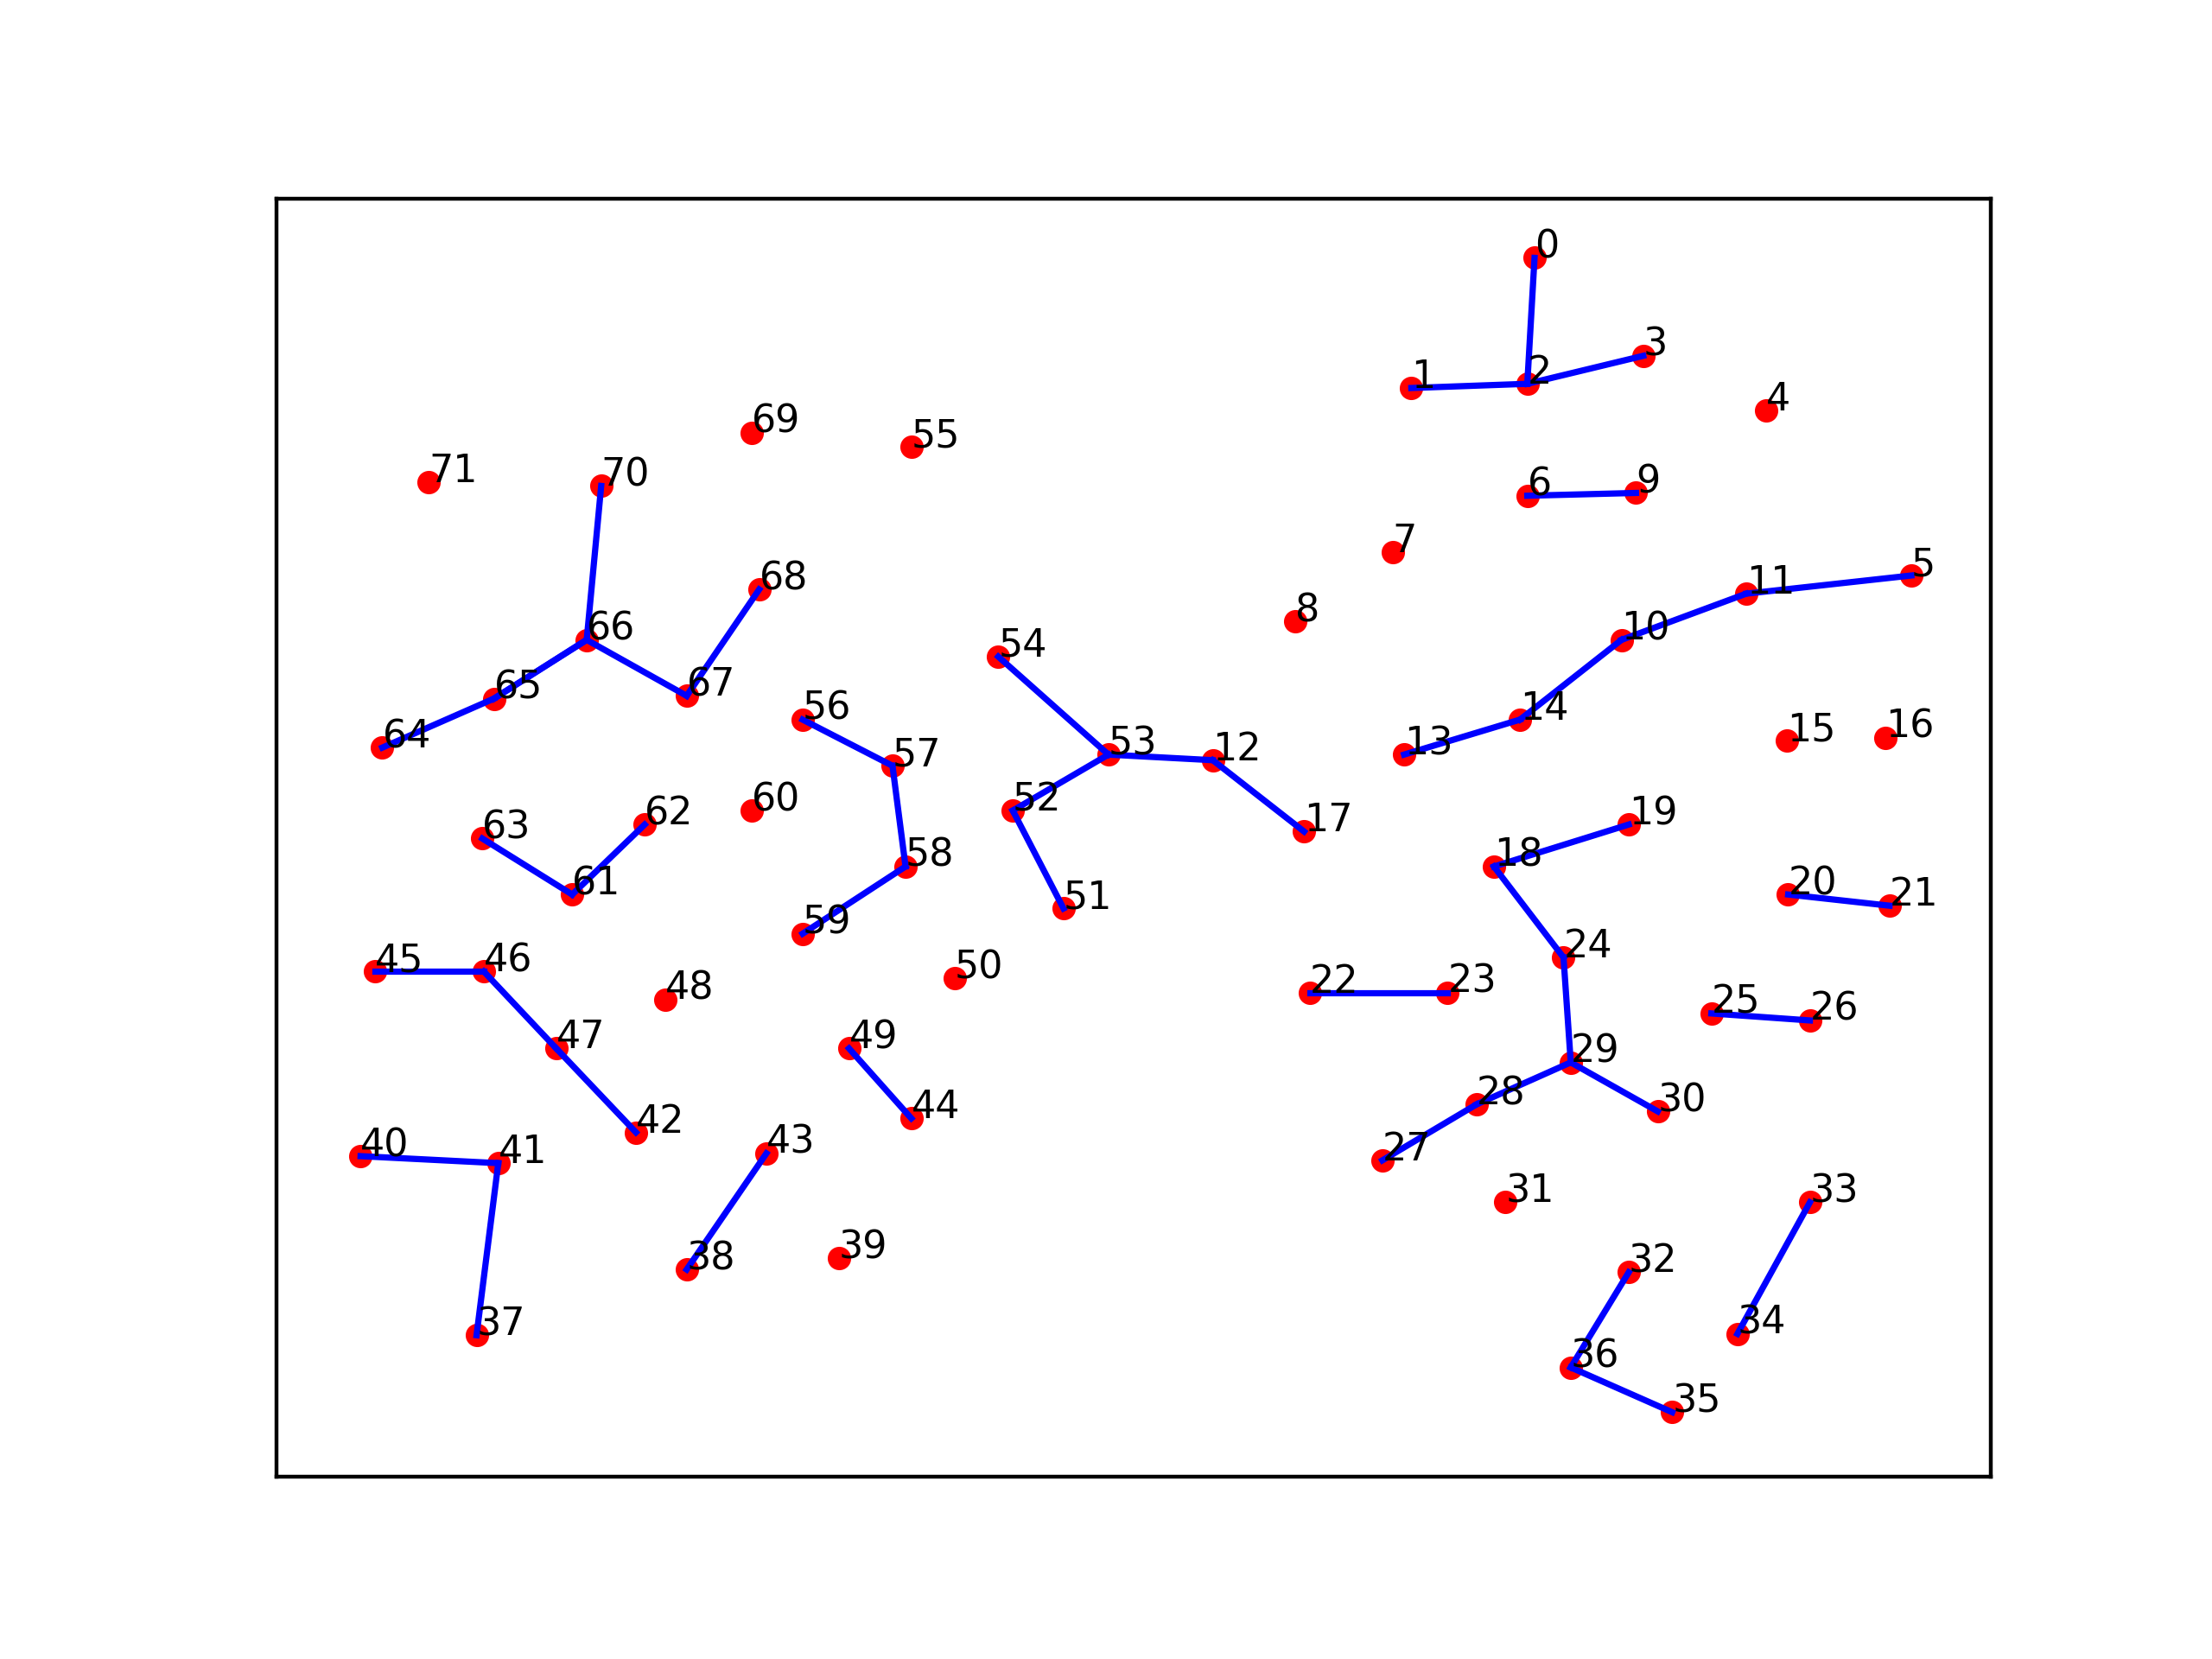
\includegraphics[scale=.5]{2_step2.png}\vspace{4pt}
	        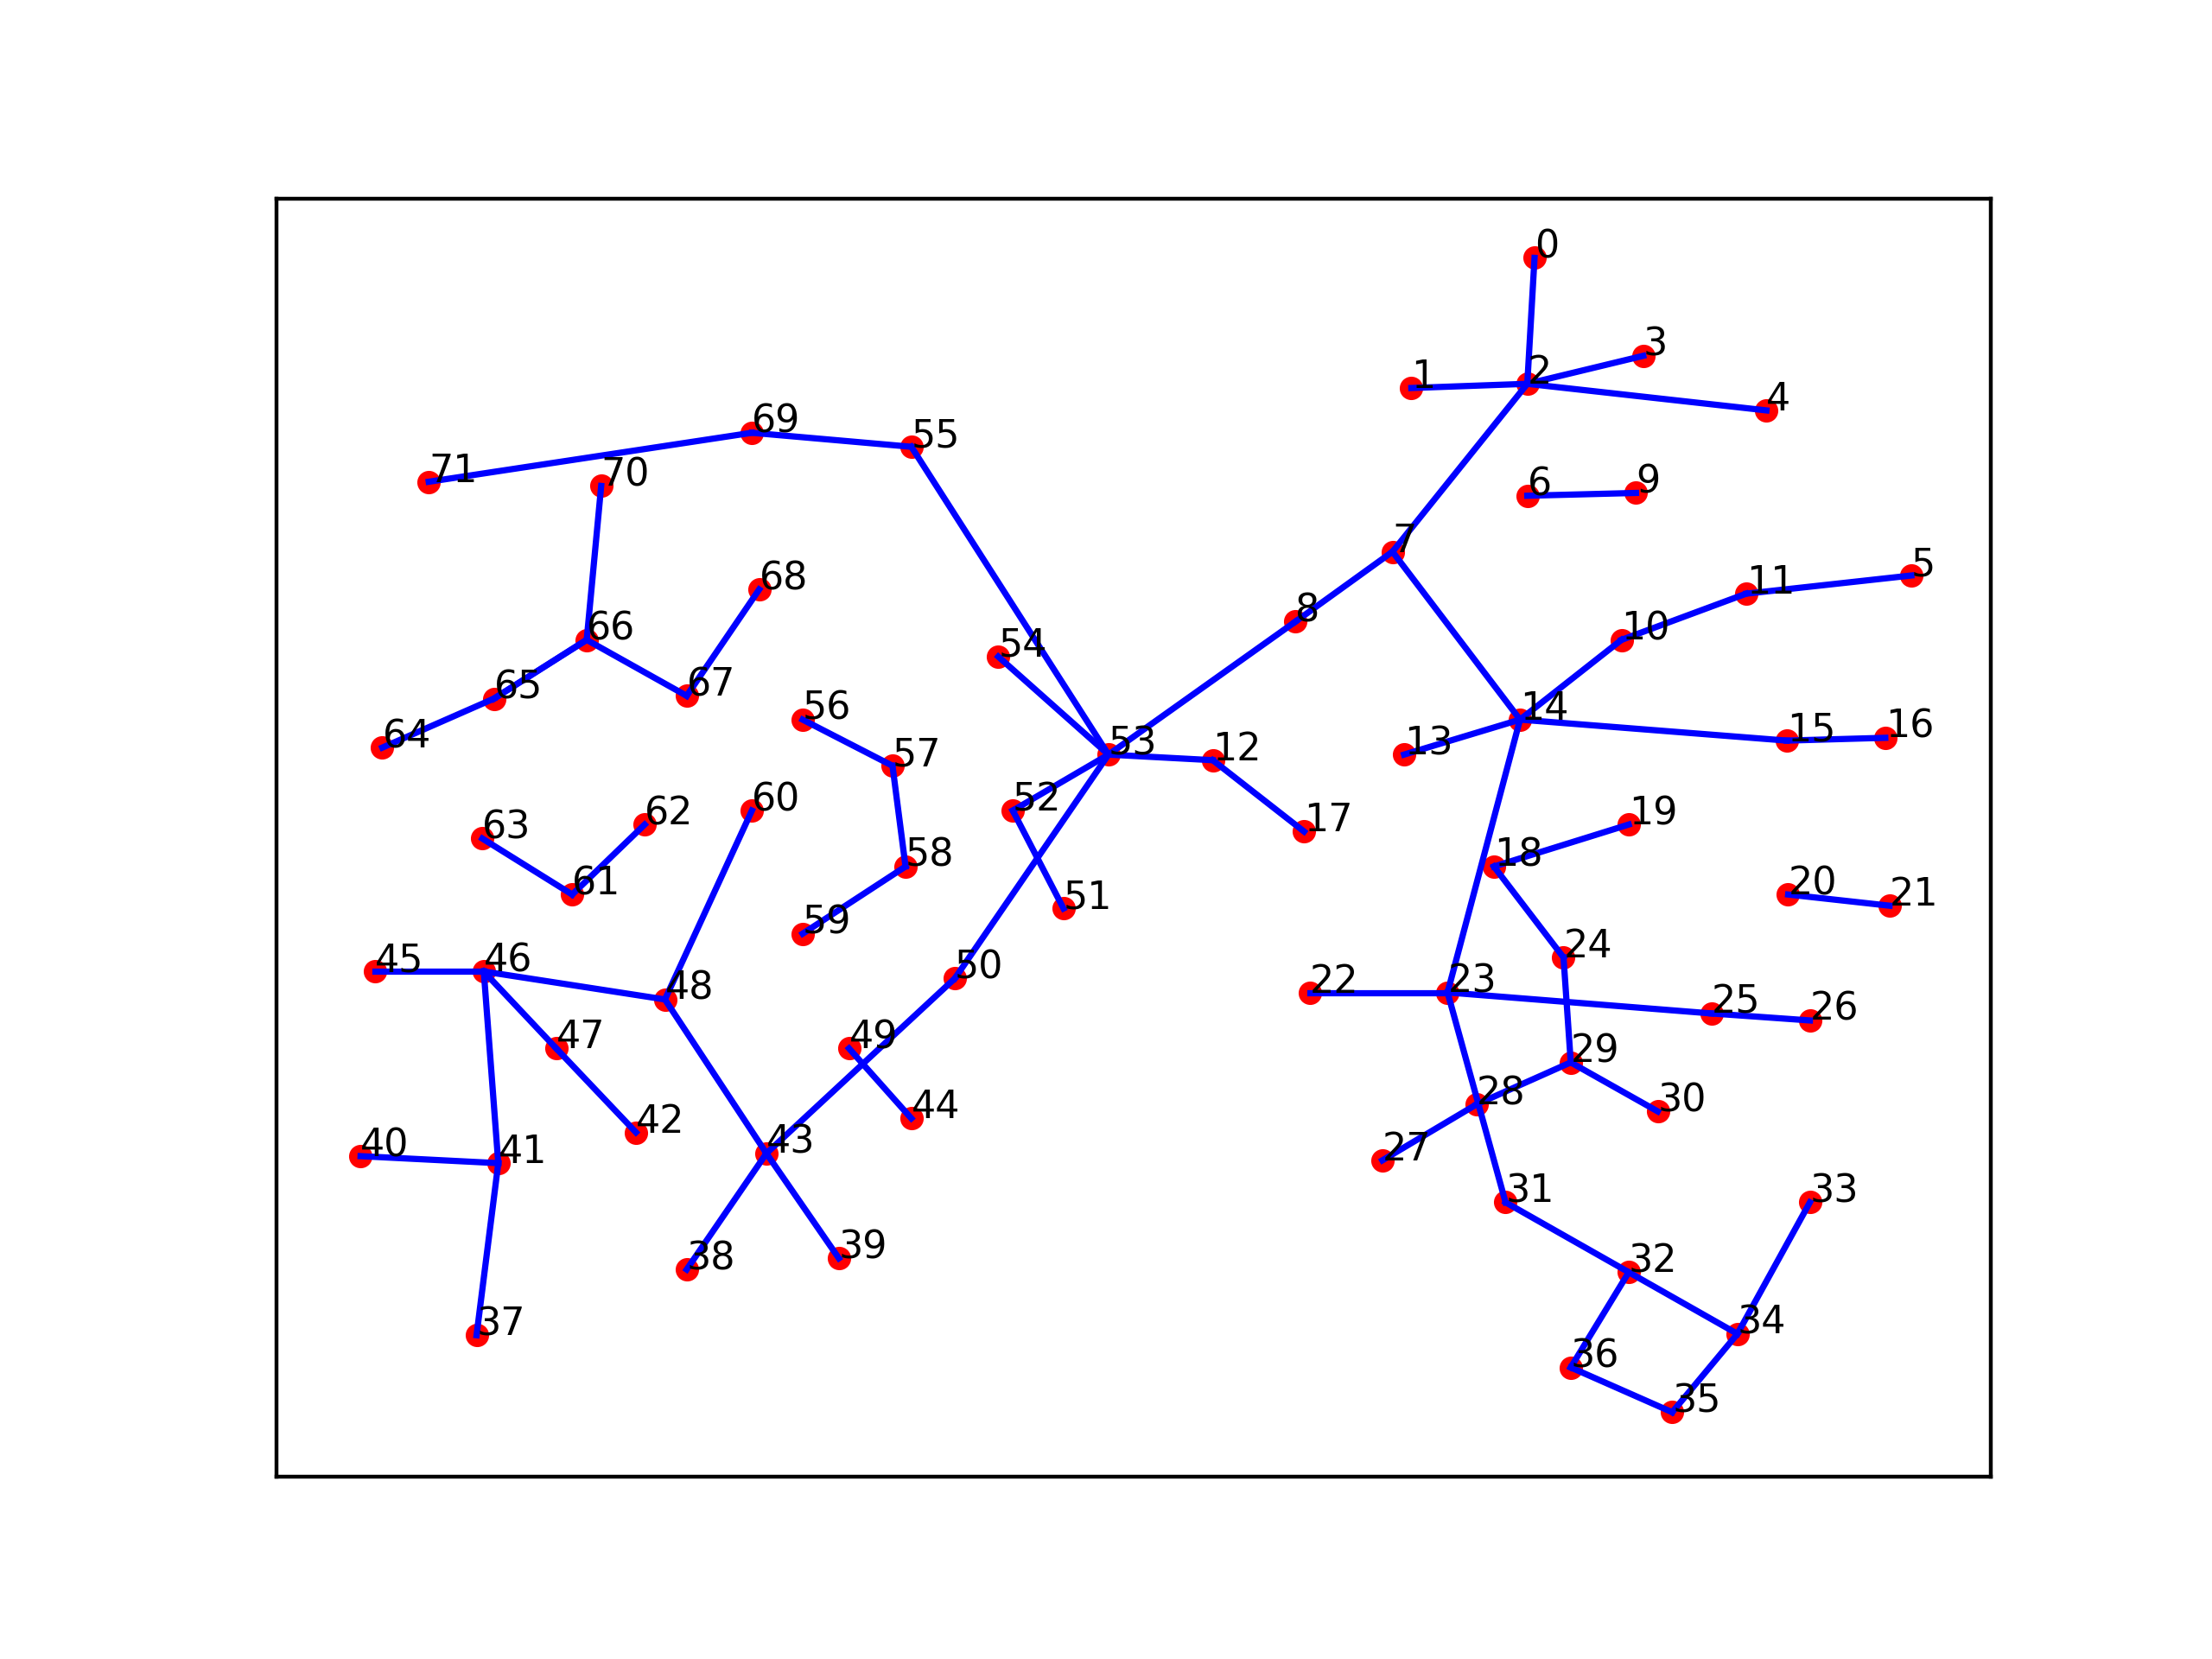
\includegraphics[scale=.5]{2_step3.png}\vspace{4pt}
	        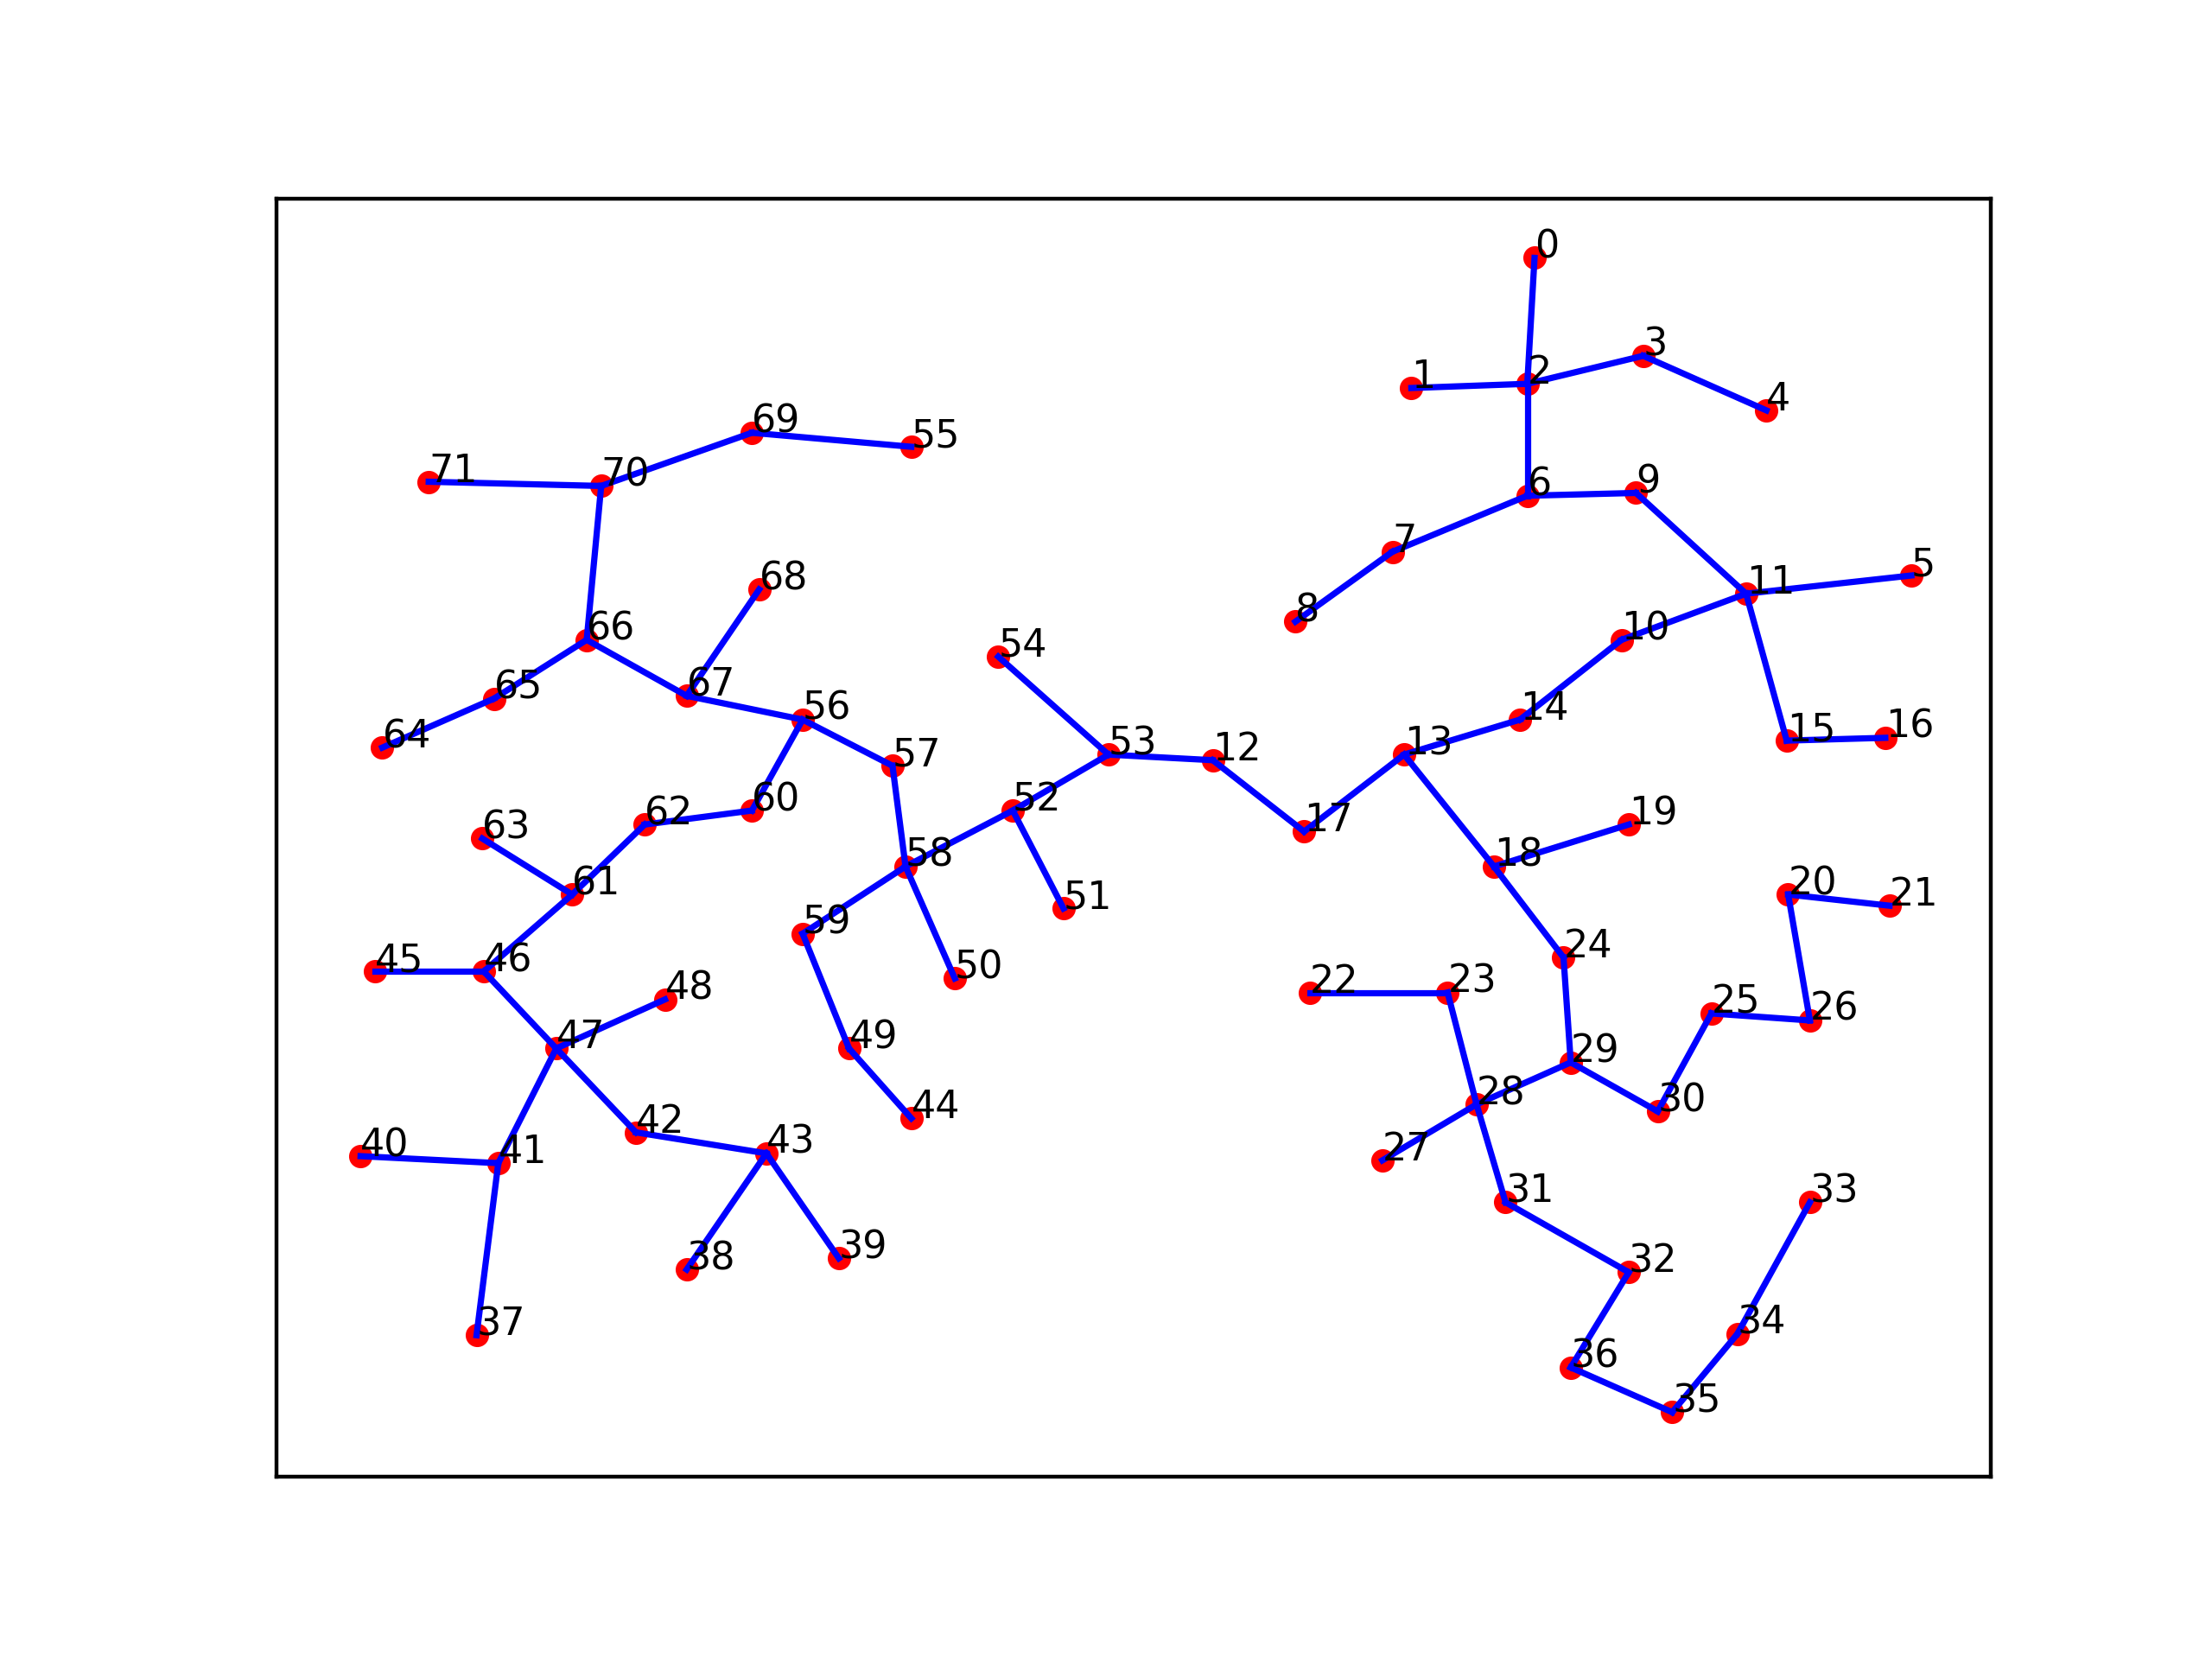
\includegraphics[scale=.5]{2_step4.png}
	        % \vspace{-2cm}
	        \caption{steps of our second Sampling-based MST algorithm}
	    \end{figure}
		
	\subsection{AMST method}
